% test.tex
\title{Policy Gradient vs. Action-Value Methods on Stochastic and Non-Stochastic Environments}

\author{M Bedir Tapkan}

\newcommand{\abstractText}{\noindent
	In this report I present an experiment that compares and contrasts the differences between action-value and policy gradient methods. In particular, the experiments evaluate the performances of both methods on stochastic and non-stochastic environments. The results demonstrate that policy gradient methods are not actually outperforming action-value based methods in stochastic environments. Even though that is the case, increasing stochasticity seems to make policy gradient methods relatively better. On the other hand, action-value based method used, outperforms the policy gradient method by a large margin on the deterministic environment.
}

%%%%%%%%%%%%%%%%%
% Configuration %
%%%%%%%%%%%%%%%%%

\documentclass[10pt, letterpaper, twocolumn]{article}
\usepackage{xurl}
\usepackage[super,comma,sort&compress]{natbib}
\usepackage{abstract}

\usepackage{graphicx}
\graphicspath{ {imgs/} }

\renewcommand{\abstractnamefont}{\normalfont\bfseries}
\renewcommand{\abstracttextfont}{\normalfont\small\itshape}

\usepackage{algorithm}
\usepackage{algorithmic}

\usepackage{bm}
\usepackage{enumitem,amssymb}
\newlist{todolist}{itemize}{2}
\setlist[todolist]{label=$\square$}

% Any configuration that should be done before the end of the preamble:
\usepackage{hyperref}
\hypersetup{colorlinks=true, urlcolor=blue, linkcolor=blue, citecolor=blue}

\begin{document}
	
	%%%%%%%%%%%%
	% Abstract %
	%%%%%%%%%%%%
	
	\twocolumn[
	\begin{@twocolumnfalse}
		\maketitle
		\begin{abstract}
			\abstractText
			\newline
			\newline
		\end{abstract}
	\end{@twocolumnfalse}
	]
	
	%%%%%%%%%%%
	% Article %
	%%%%%%%%%%%
	
	\section{Introduction}
	
	\normalsize 
	\noindent Section 13.1 of \textit{Reinforcement Learning: An Introduction}(Sutton and Barto, 2018) outlines a number of potential advantages of policy-gradient methods over value based methods. Of these advantages, one of the most important, and personal interest to me, is \textit{stochasticity}. Due to the fact that action-value methods are incapable of finding a stochastic optimal policy, policy-gradient methods should perform better in stochastic environments. I find this distinction particularly interesting, and wanted to further explore this benefit of policy-gradient methods for my report.\\
	
	In order to test the proposition that policy-gradient methods should outperform action-value methods in a stochastic environment, I created two environments in which to train the algorithms, one stochastic and one non-stochastic. The stochastic and non-stochastic environments have similar designs in order to make an effective comparison of the algorithms. For the experiment, I selected representative algorithms for policy-gradient methods and action-value methods. I compared the algorithms \textit{REINFORCE} (a basic policy gradient algorithm) and \textit{Episodic Semi-Gradient SARSA}(a basic action-value based algorithm). The design of the experiment attempted to ensure that the stochasticity of the environment would be the only variable that would have an effect on algorithmic performance. \\
	
	As a result I found that action-value based methods can find optimal policy in stochastic environment, when there is a certain degree of randomness, and that policy gradient methods might not actually be working that better in comparison to action-value methods.
	
	\section{Environment}
	%\small \textit{This section is included only for the first report, it will not be included in the following ones. It will only include a summary of what the project is.}\\
	
	\noindent \textbf{Base} The environment used in the experiment is a basic grid world system. Grid worlds refer to a range of problems where the agent is allowed to take an action and move through the world. The main goal of the agent is often to reach a specific position in the grid world (this was done in my experiments for this report), but agent could also have a variety of other goals (e.g. try to stay alive as long as possible). The defining feature of grid worlds is that the environment is composed of blocks and the agent can move from one block to another. The movement rules and action space can vary depending on the agent's location or specific choices for the construction of the grid world. For example, the agent might be allowed to move only right and left as is the case in a specific version of grid world known as chain environment (name does not matter, it just is a grid world with two actions). Alternatively, the agent may be able to move in all four cardinal directions, as in the famous Atari game 'Bomberman'.\\
	
	\noindent \textbf{Specific} The environments created for the experiment are based on simple grid world rules with a few additional adjustments. The agent is allowed to move in all four cardinal directions (North, South, East, West). The environment is composed of a static starting position, where the agent begins, and a goal position. As is commonly used in grid worlds, the agent receives a reward of $-1$ for each time step that is spent before reaching its goal, and if the goal is reached, the agent receives a reward of $+10$. If the agent attempts to make an invalid move (i.e. hitting an obstacle, such as a wall), it remains in the same position, but will still receives a reward of $-1$. 
	
	\begin{figure}[h]
		\centering
		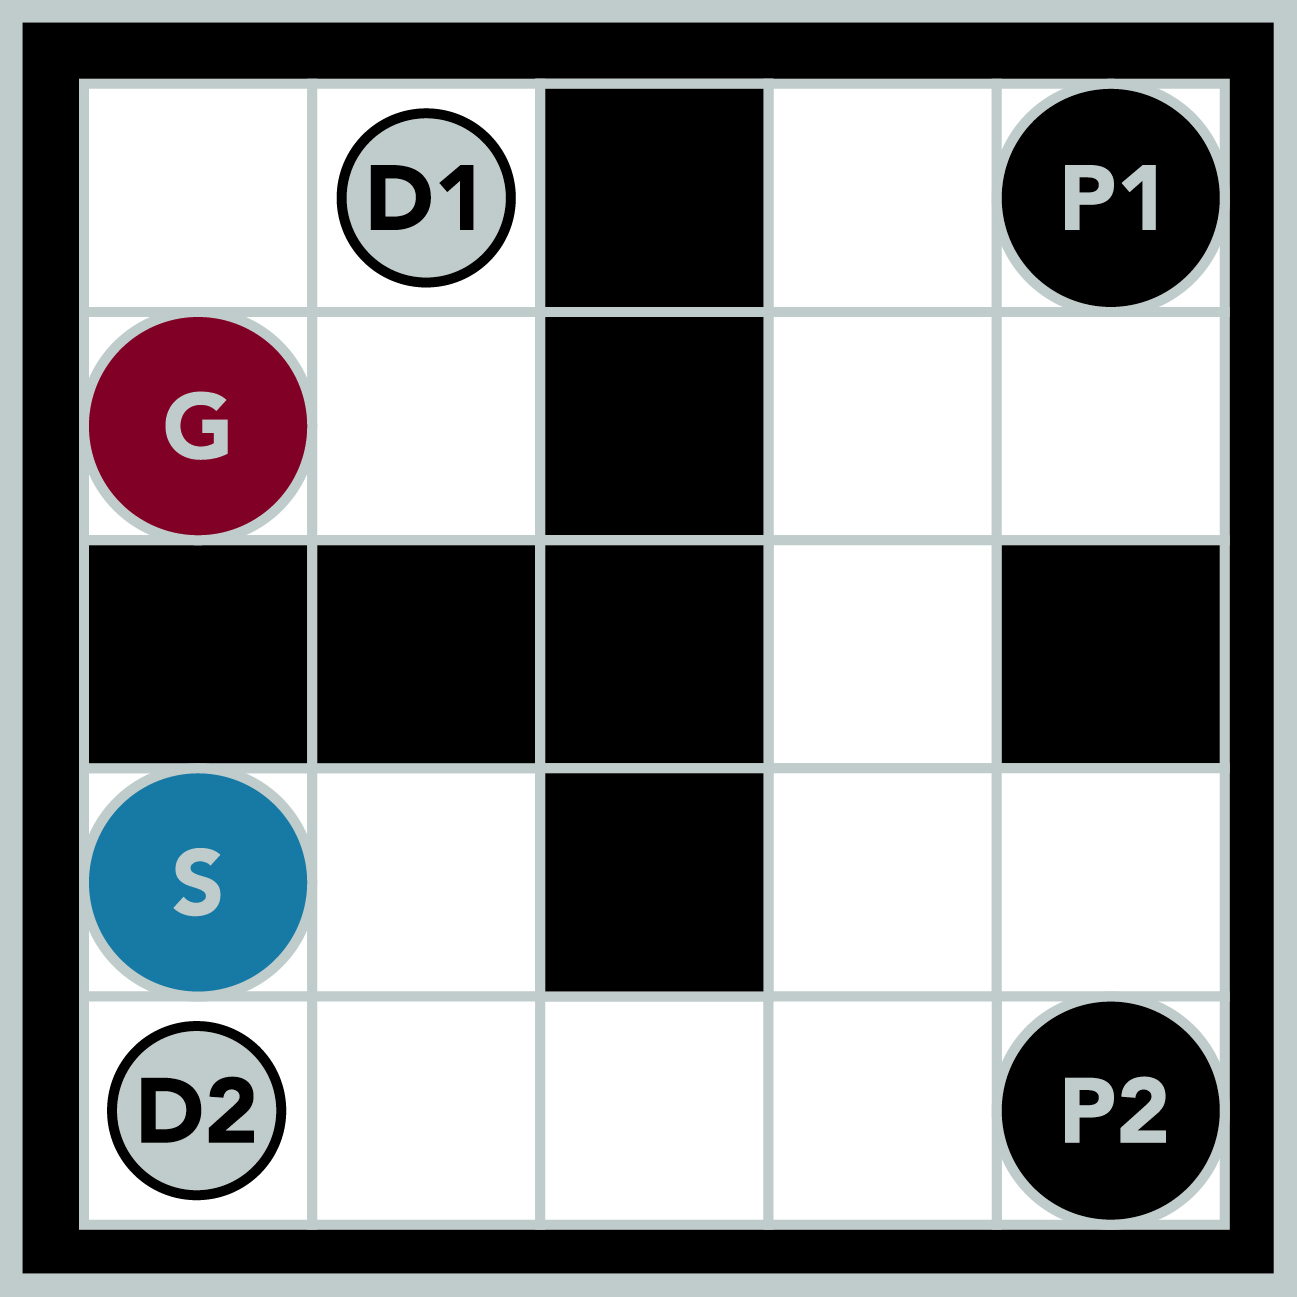
\includegraphics[width=0.49\linewidth]{grid_2x2}
		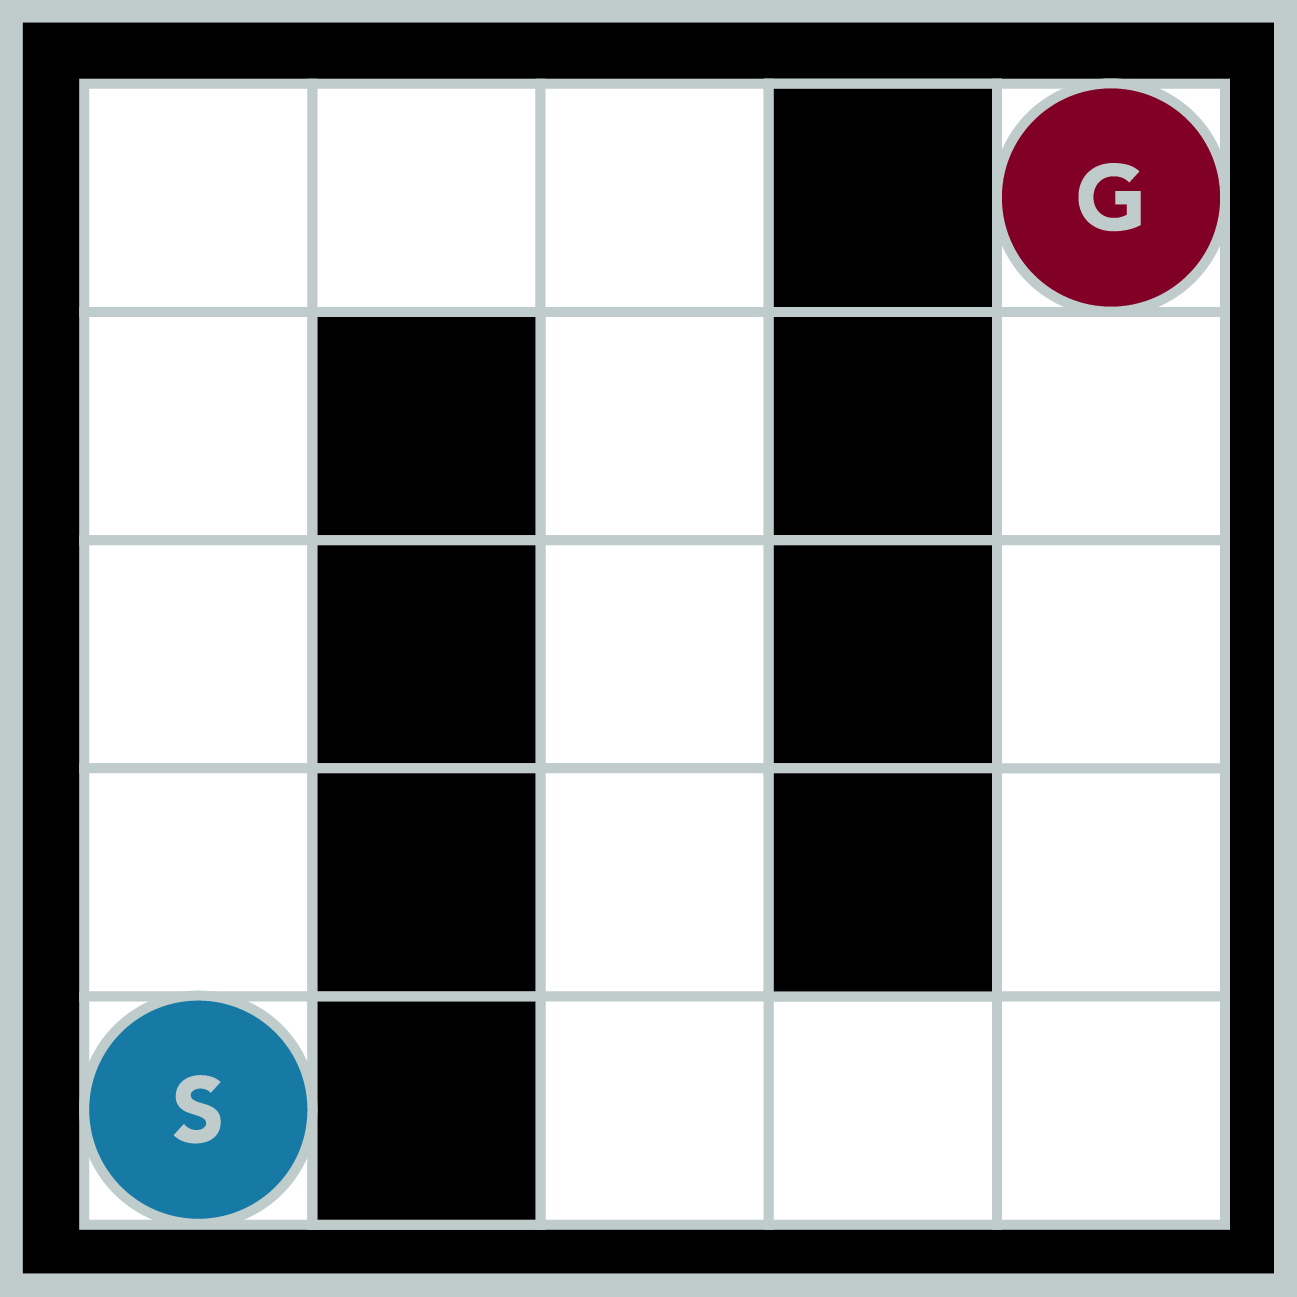
\includegraphics[width=0.49\linewidth]{grid_2x2_det}		
		\caption{\small The grid worlds used in experiment 1 and 2. The image on the left represents the stochastic environment and the image on the right represents the deterministic environment. The agent starts from position $S$ and attempts to reach position $G$. Black boxes are obstacles. Other materials are explained below.}
		\label{fig:grid_world}
	\end{figure}
	
	\noindent \textbf{The rest} The stochastic and non-stochastic environments are shown in Figure \ref{fig:grid_world}. As shown in the figure, environments contain some additional features to help with the experiment. These features are defined here:
	\begin{itemize}
		\item \textbf{P1:} Portal 1. The portals transfer the agent from one location to another. Each portal has a pre-determined destination point. With probability $p_1 = 0.6$ \textbf{P1} teleports the agent to \textbf{D1}, and with probability $p_2 = 0.4$ it teleports the agent to\textbf{D2}.
		\item \textbf{P2:} Portal 2. \textbf{P2} teleports the agent to the agent to whichever destination \textbf{P1} has not been assigned. 
		\item \textbf{D1:} Destination point 1. The portals (defined above) transfer the agent to destination points.
		\item \textbf{D2:} Destination point 2. 
	\end{itemize}
	
	As can be seen in the figure above, in order to reach the goal point in the stochastic environment, the agent must be teleported to \textbf{D1}. Therefore, the agent must first reach \textbf{P1} or \textbf{P2} to be teleported to \textbf{D1}, from which it will be able to move further and finally reach the goal.\\
	
	\noindent \textbf{What's special?} The stochastic and non-stochastic environments are distinguished by the behavior of the portals. The stochasticity comes from the portals. After each usage of either \textbf{P1} or \textbf{P2}, the destinations are randomly re-initialized according to the probabilities above. The deterministic environment (image on the right of the figure) clearly has no stochasticity, as the agent only needs to follow the corridor in order to reach the goal.
	
	\section{Algorithms}
	
	\noindent There are two algorithms compared in both environment tasks. As mentioned before, the experiments aim to compare action-value methods with policy gradient methods. To this end, I chose a policy gradient algorithm that seems to be a good fit for this comparison, and then an action-value based algorithm that is comparable with the chosen method.
	
	\subsection{Policy Gradient: REINFORCE}
	\noindent REINFORCE stands for \textit{"REwardIncrement = NonnegativeFactor $\times$ OffsetReinforcement $\times$ CharacteristicEligibility"}. It was proposed by Ronald J. Williams (Williams, 1992). It is one of the first policy gradient methods proposed, and is a Monte-Carlo Policy Gradient method. \\
	
	\noindent \textbf{Why REINFORCE?} REINFORCE was chosen for the experiment because it is a policy gradient method which does not use values to update the policy. I chose not to use baselining (a related policy gradient method, based on REINFORCE) as it makes use of value updates. Hence, the central rationale for choosing REINFORCE was because I wanted a clear distinction between my policy gradient method and value based methods, and this algorithm seems to be the best fit for the purpose.
	
	\subsubsection{How does it work?}
	I will attempt to give the main idea of the algorithm and will not go into much detail here. Additional information and further detail can be found in \textit{Reinforcement Learning: An Introdcution} (Section 13.3). The update formula used for the algorithm is:
	
	$$\theta_{t+1} = \theta_{t} + \alpha \gamma^t G_t \frac{\nabla \pi(A_t| S_t, \theta_t)}{\pi(A_t| S_t, \theta_t)}$$
	
	\noindent \bm{$\theta$} is the weights we use for the action selection (policy). In our case,we will use the Softmax policy (formula 13.2 in the textbook). As we update our weights, we are giving more importance to the action that seems best, given the state in time $t$. Also $\theta \in \mathbb{R}^{d'}$, where $d'$ is the state representation. In these experiments we use tile coding for state representation. Details can be found in Chapter 9.\\ 
	
	\noindent \bm{$\alpha$} is the learning rate. The learning rate is a centrally important element of gradient based functions. In our case it has a really important effect, as we do not need the expected value of the samples to exactly match the gradient of the performance measure $J(\theta)$. Additional information can be found in the first paragraph of section 13.3.\\
	
	\noindent \bm{$\gamma$} is the discount factor. It is a predetermined value (meta-parameter, i.e. $0.99$).\\
	
	\noindent \bm{$G_t$} is the discounted episodic return. It is merely a basic calculation of the discounted future rewards used as the Monte Carlo target value. The formula for it is:
	
	$$G_t = \sum_{i=t+1}^{T} \gamma^{i-t-1} R_i$$
	
	Where $T$ is the terminal state time.\\
	
	\noindent The main part of the algorithm is the gradient of the policy, over the policy itself. First we can simplify this term as it is the same as the gradient of the log function.
	
	$$\frac{\nabla \pi(A_t| S_t, \theta_t)}{\pi(A_t| S_t, \theta_t)} = \nabla\ln\pi(A_t|S_t,\theta_t)$$
	
	After we have this, for the softmax policy we have a simple form to use (exercise 13.3 in the textbook):
	
	$$\nabla\ln\pi(a|s,\theta) = x(s,a) - \sum_{b}\pi(b|s, \theta)$$
	
	Complete pseudo code for the algorithm used is given in Algorithm 1 below.
	
	
	\begin{algorithm}
		
		\caption{REINFORCE}
		\begin{algorithmic}
			\FOR{each episode}
			\STATE Generate a trajectory using the policy $S_0, A_0, R_1,\ldots, S_{t-1}, A_{t-1}, R_t$
			\FOR{each step t [0, T)}
			\STATE $G \leftarrow \sum_{i=t+1}^{T} \gamma^{i-t-1} R_i$
			\STATE $\theta \leftarrow \theta + \alpha G \gamma^{t} \nabla\ln\pi(A_t|S_y, \theta)$
			\ENDFOR
			\ENDFOR
		\end{algorithmic}
	\end{algorithm}
	
	\subsection{Semi-gradient SARSA}
	
	\noindent \textbf{Why Semi-gradient SARSA?} The goal of the experiment is to compare policy gradient and action-value based methods, so the choice of algorithm reflects this goal. In an attempt to restrict the variability of the algorithms to the difference in methods, i.e. policy gradient versus action-value, I needed the value-based algorithm to be as similar to REINFORCE as possible. Since REINFORCE uses Monte-Carlo updates, and the task at hand is episodic, I chose the simplest algorithm that fits this scheme. 
	
	Semi-gradient SARSA is a control algorithm that can use Monte Carlo update. Because of this I used Episodic semi-gradient SARSA, as given in chapter 10 of the textbook.
	
	\section{Experiment}
	
	\subsection{Assumptions and Hypothesis}
	
	\noindent As the title suggests, my aim was to investigate how stochasticity in an environment effects the results in policy gradient methods versus value-based methods. Theoretically, policy gradient methods should have superior performance in stochastic environments, so my hypothesis was that the policy gradient method (REINFORCE) would perform significantly better in the stochastic environment than the action-value based method (SARSA). For the deterministic environment I also expected REINFORCE to perform better than SARSA, but I expected the performance of the two algorithms to be more similar in this environment.\\
	
	\subsection{The path followed}
	
	\noindent I used the first environment (stochastic) for experiment 1, and the second environment (deterministic) for experiment 2. I attempted to control other factors that could have an effect on the algorithms' performances so that the main reason for variability in performance would be the stochasticity of the environment. \\
	
	\noindent \textbf{Maximum number of steps} Initially, I planned to run each episode until the terminal state, which is what is generally done for episodic cases, but since I used Monte-Carlo methods, which update the weights only at the end of an episode, the models would often take an excessively long time to reach the goal in the first episode, and thus taking an unneccesarily large amount of steps and increase the time to convergence. After the first few episodes the agent would quikcly reach the goal. Due to this I decided to put a limit on number of steps in order to train the models more efficiently. The maximum number of steps allowed per episode was $1000$, which, while still unnecessarily large, helped to stop some episodes before the terminal state. \\
	
	\noindent \textbf{Step size} I used the best domain step-size I found for both algorithms. I tested 10 step sizes for each, and used the best performing one in an average over 10 runs. Figure \ref{fig:step_size_reinforce} and \ref{fig:step_size_sarsa} shows the results of the parameter sweeping.\\
	
	\begin{figure}[h]
		\centering
		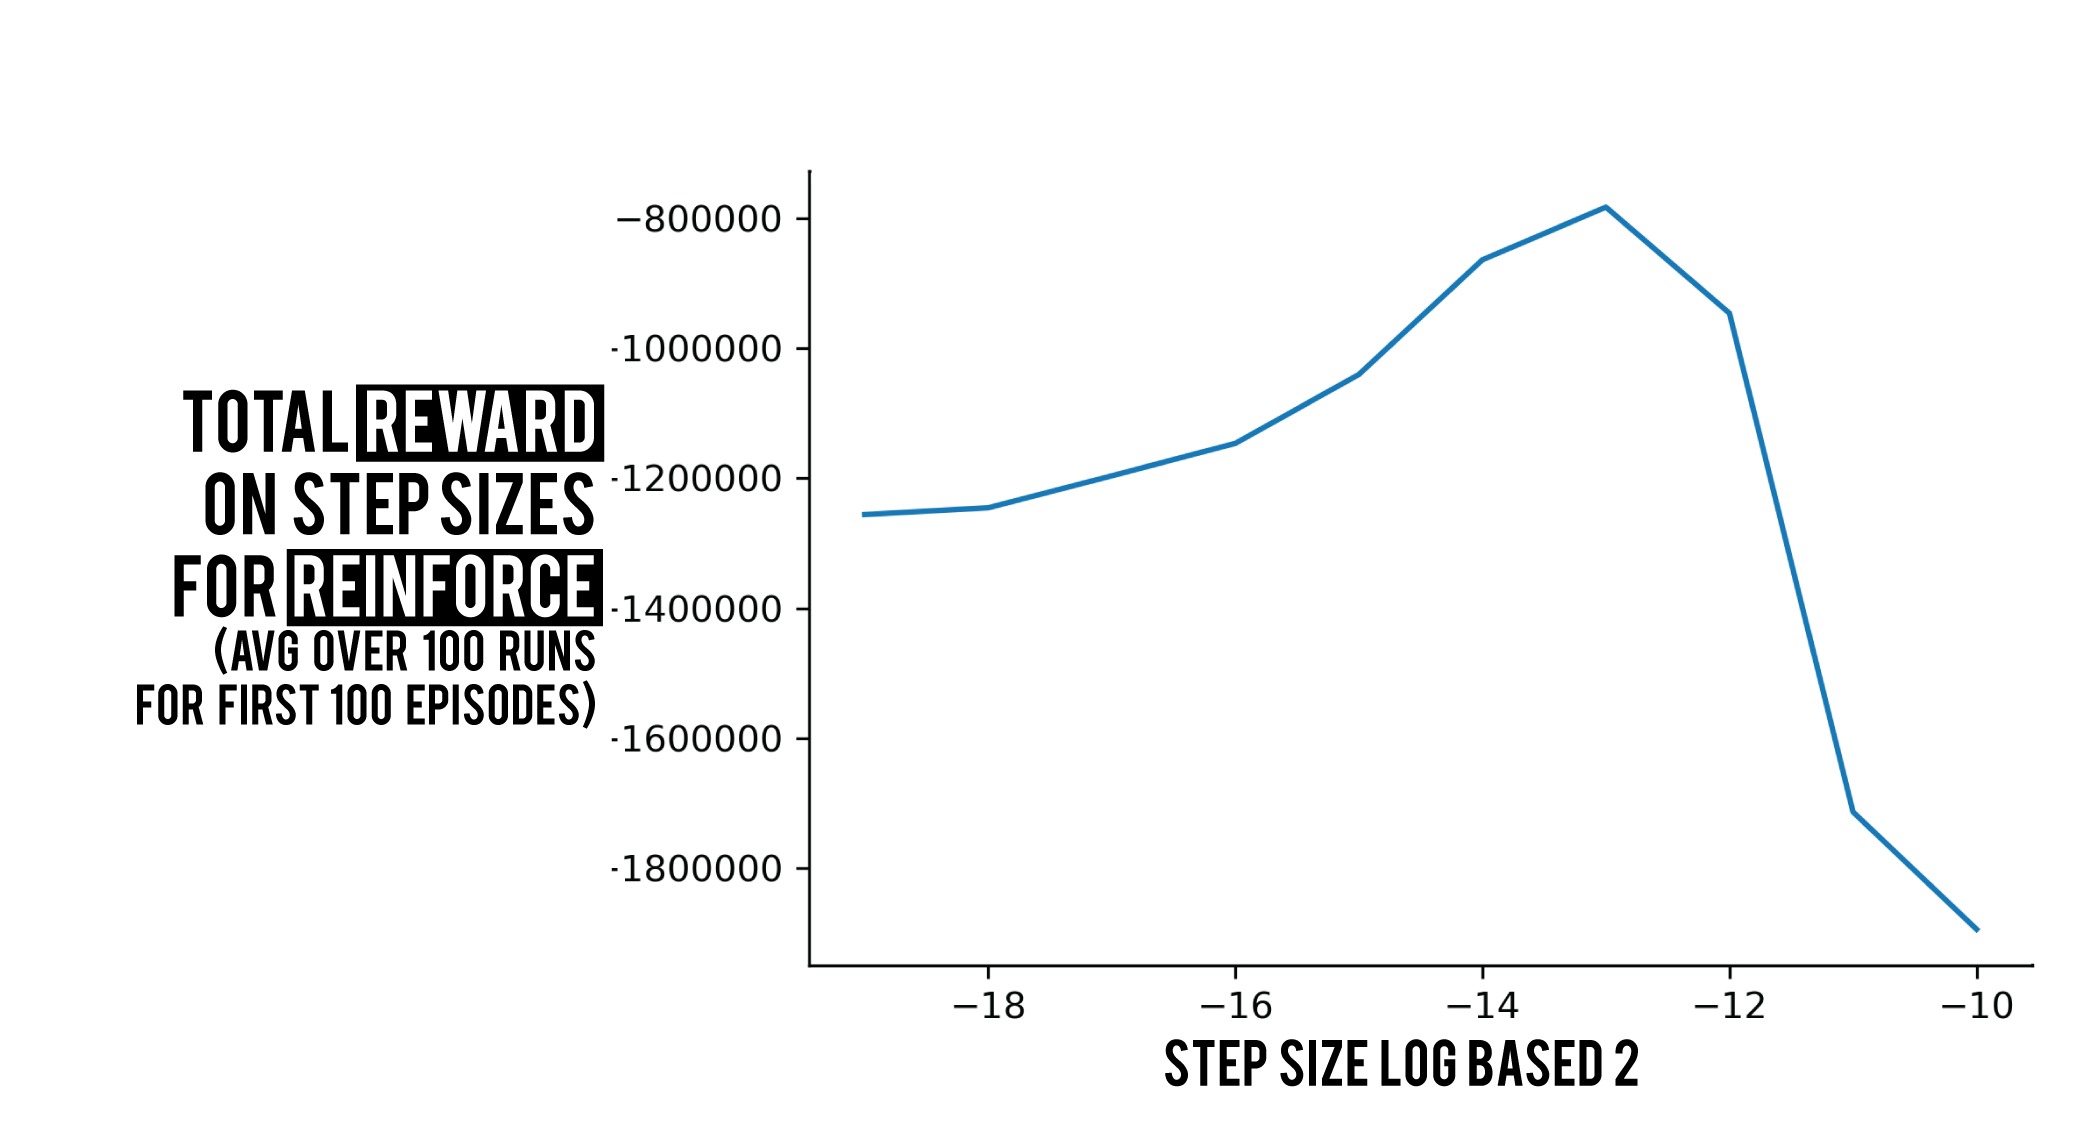
\includegraphics[width=\linewidth]{figure_parameter_reinforce}
		\caption{\small Step size analysis in the grid world for REINFORCE. As can be seen $2^{-13}$ gave the best results, which is the step size used after this point onward.}
		\label{fig:step_size_reinforce}
	\end{figure}
	
	\begin{figure}[H]
		\centering
		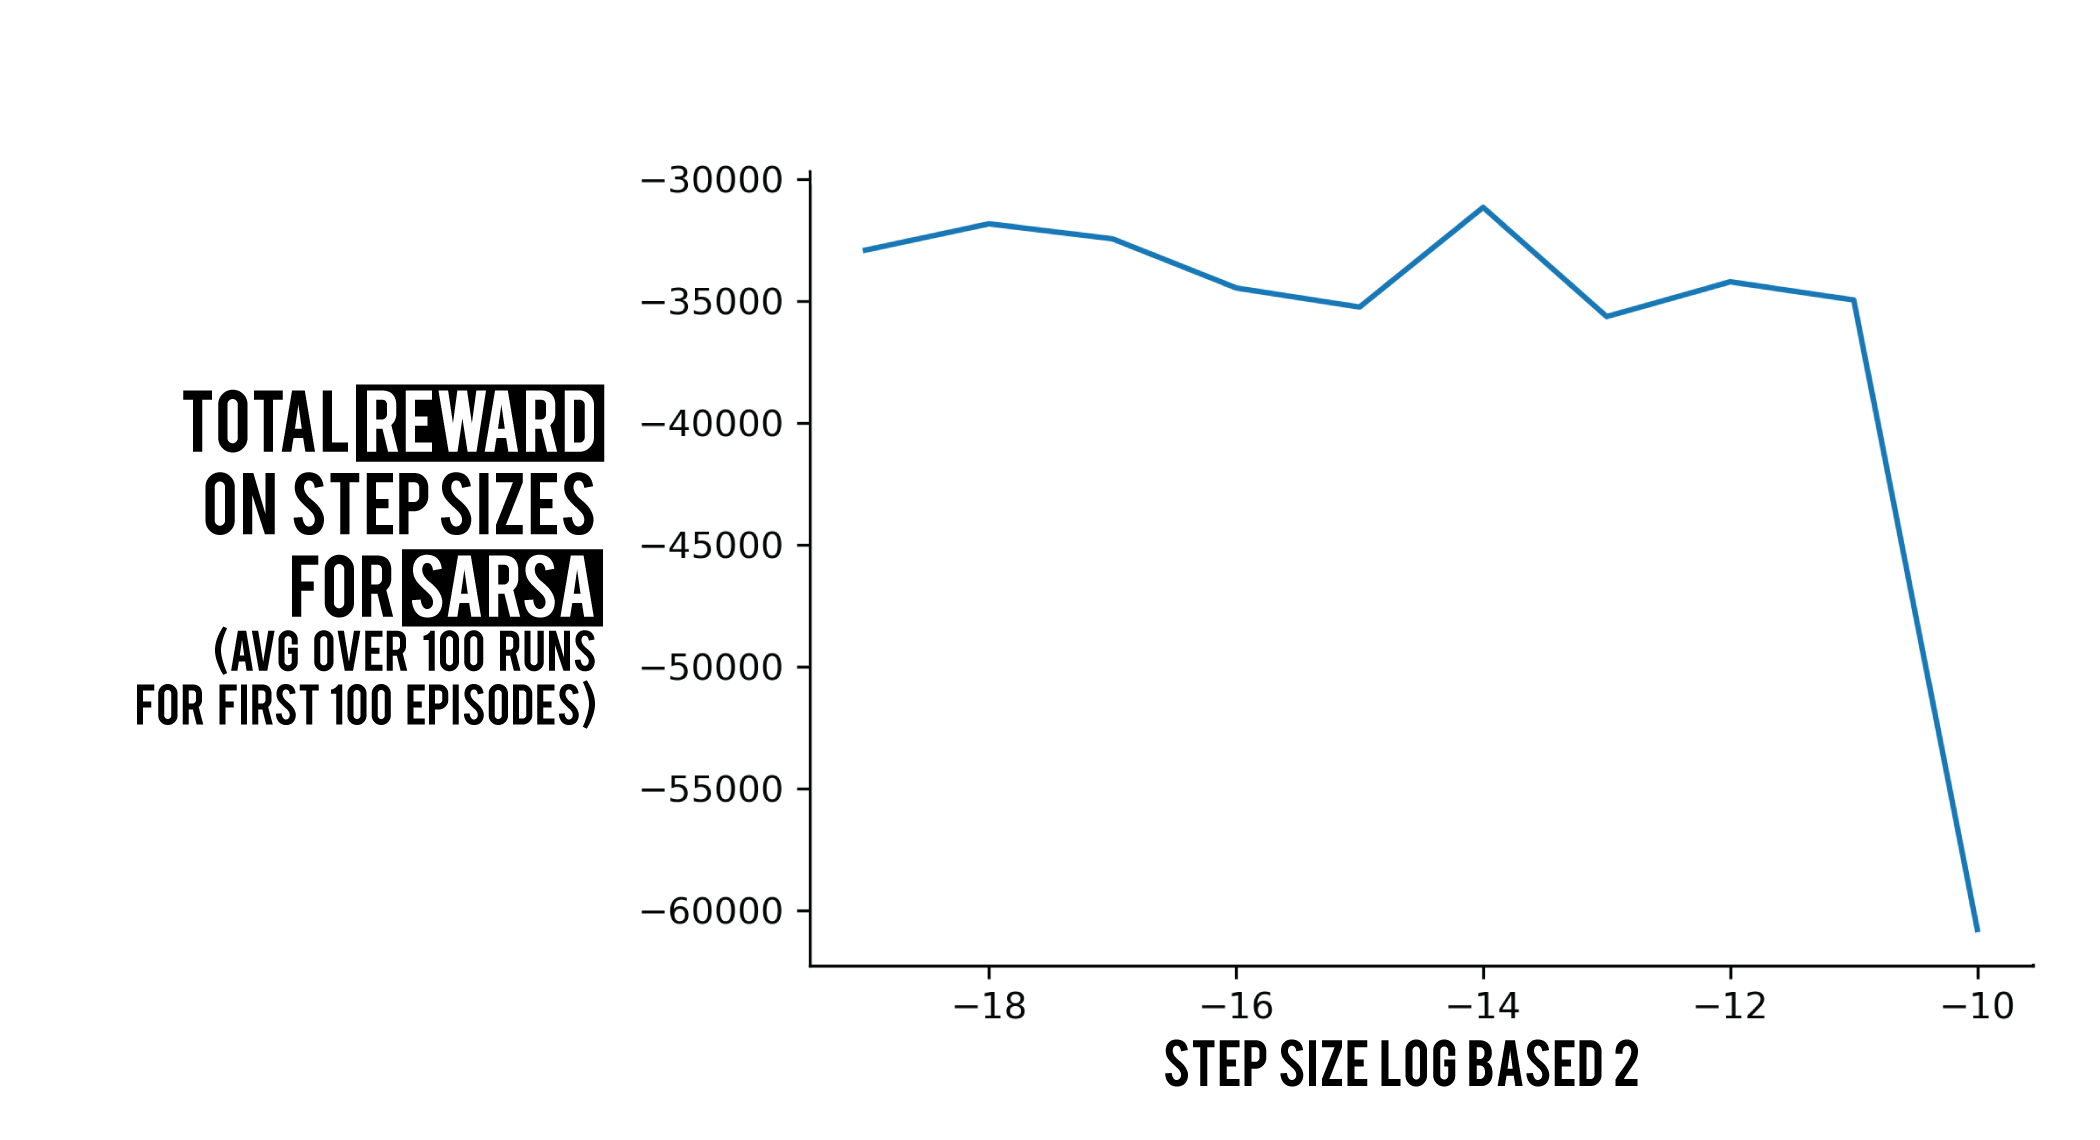
\includegraphics[width=\linewidth]{figure_parameter_sarsa}
		\caption{\small Step size analysis in the grid world for Episodic Semi-gradient SARSA. The best result is $2^{-14}$}
		\label{fig:step_size_sarsa}
	\end{figure}
	
	\noindent \textbf{Feature representation} To represent the states, I used tile coding (discussed in chapter 9 of the textbook). I used the same tilings for both algorithms. For action value representations, the tilings are concatenated after one another, for the number of actions. i.e. for state 1 if state representation is [0 1 0 0], and active action is also 1, since we have 4 possible actions the representation will be: \\
	
	[0 0 0 0 \textbf{0 1 0 0} 0 0 0 0 0 0 0 0]\\
	
	
	\noindent \textbf{Different rewards?} I also tried to vary the rewards depending on the area of the grid to speed up the learning (e.g. a higher penalty for spending more time steps occupying cells in the lower left quadrant of the grid). After experimenting with this I decided that this made the task to easy for the agent and this line of experimentation was abandoned. \\
	
	\noindent \textbf{Randomness} In order to ensure randomness in my experiments, I used a different seed for each run, and averaged all the results together.
	
	\subsection{Reproducing the Results} 
	
	\noindent The results are easily reproducible once all the hyper-parameters are set correctly. The following provides the necessary information to reproduce the results.
	
	\subsubsection{Experiment 1 and 2}
	
	\noindent There was total of 100 runs for each algorithm, and the results acquired in each episode is averaged over these 100 runs.\\
	
	\noindent \textbf{Seeding} Seed numbers are important to reproduce the given results since the randomness depends on them. For each run I used the seed number $r+1$ where $r$ is the run index. For example, for the first run the index is 0, therefore the seed number will be 1.\\
	
	\noindent \textbf{Step Size} A constant, and set to $\alpha = 2^{-13}$ for REINFORCE and $\alpha = 2^{-14}$ for SARSA.\\
	
	\noindent \textbf{Maximum steps} Number of steps the agent can take in each episode. Also a constant - set to 1000. \\
	
	\noindent \textbf{Number of episodes} A constant, 1000 episodes for each run. \\
	
	\noindent \bm{$\gamma$} Discount factor, constant  $= 0.98$.\\
	
	\noindent \textbf{Tile Coding} I used two tilings with each tile of size 2. Starting points of the tiles are 0,0 and 1,1. Therefore we have 18 tiles for states in total. Refer to Figure \ref{fig:tile_coding} to see all of the tiles created along with the corresponding cell positions.
	
	\begin{figure}[h]
		\centering
		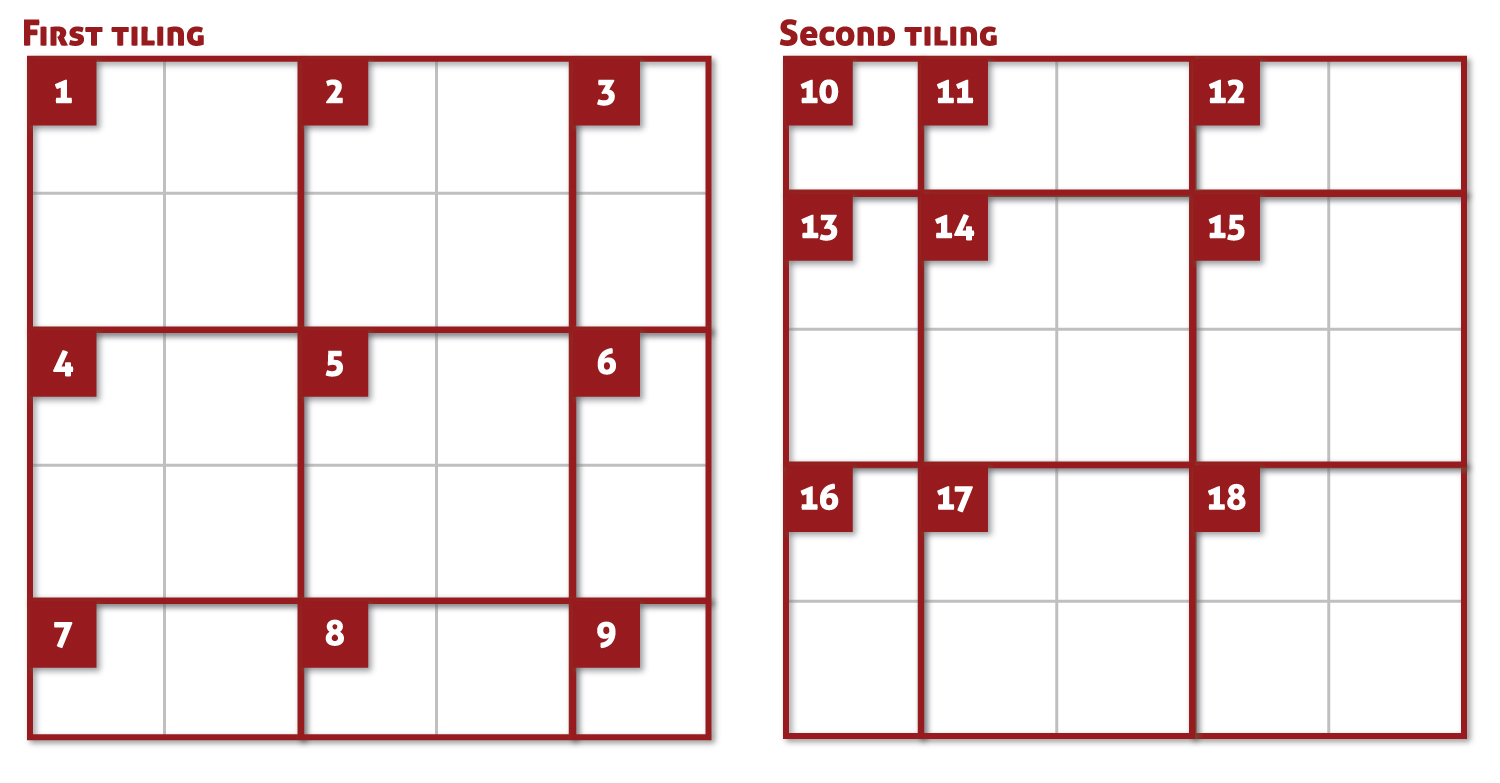
\includegraphics[width=\linewidth]{tiles}
		\caption{\small Both tilings used for the experiments. As can be seen each cell in the grid world activates two tiles from both different tilings. For example, grid location 0,0 (left-most top cell) is in tile 1 and tile 10 therefor those tiles will be activated when the agent is in position 0,0}
		\label{fig:tile_coding}
	\end{figure}
	
	\noindent \textbf{Stochasticity} As mentioned in the environment section, there are no portals in experiment 2, and therefore no randomness. To reproduce the results make sure that the probabilities of the portals are the same (60-40).
	
	\subsubsection{Parameter Study}
	
	\noindent In case this study is also of interest I will add a short setup for this as well. \\
	
	\noindent Every parameter was the same as the experiments 1 and 2, except the step sizes which was as mentioned changing on each parameter run. There was 5 total runs for both SARSA and REINFORCE. \\
	
	\noindent For both algorithms the tested values were $a_t = {2^{-10},\ldots,2^{-20}}$.\\
	
	\subsubsection{Extensions}
	
	\noindent There are couple extensions to the experiments. For both extensions, to increase the randomness wind added. For the first one there is the random chance with the probability of $p = 0.2$, and for the second extension this probability goes up to $p = 0.5$.

	\subsection{Results}
	
	The results were not as I expected. For the first experiment the results are showing that SARSA and therefor action-value methods are better than policy gradient methods for deterministic environments. Which was what I expected as I stated in my hypothesis. Figure \ref{fig:deterministic} shows the results for the experiment 1. 
	
	\begin{figure}[h]
		\centering
		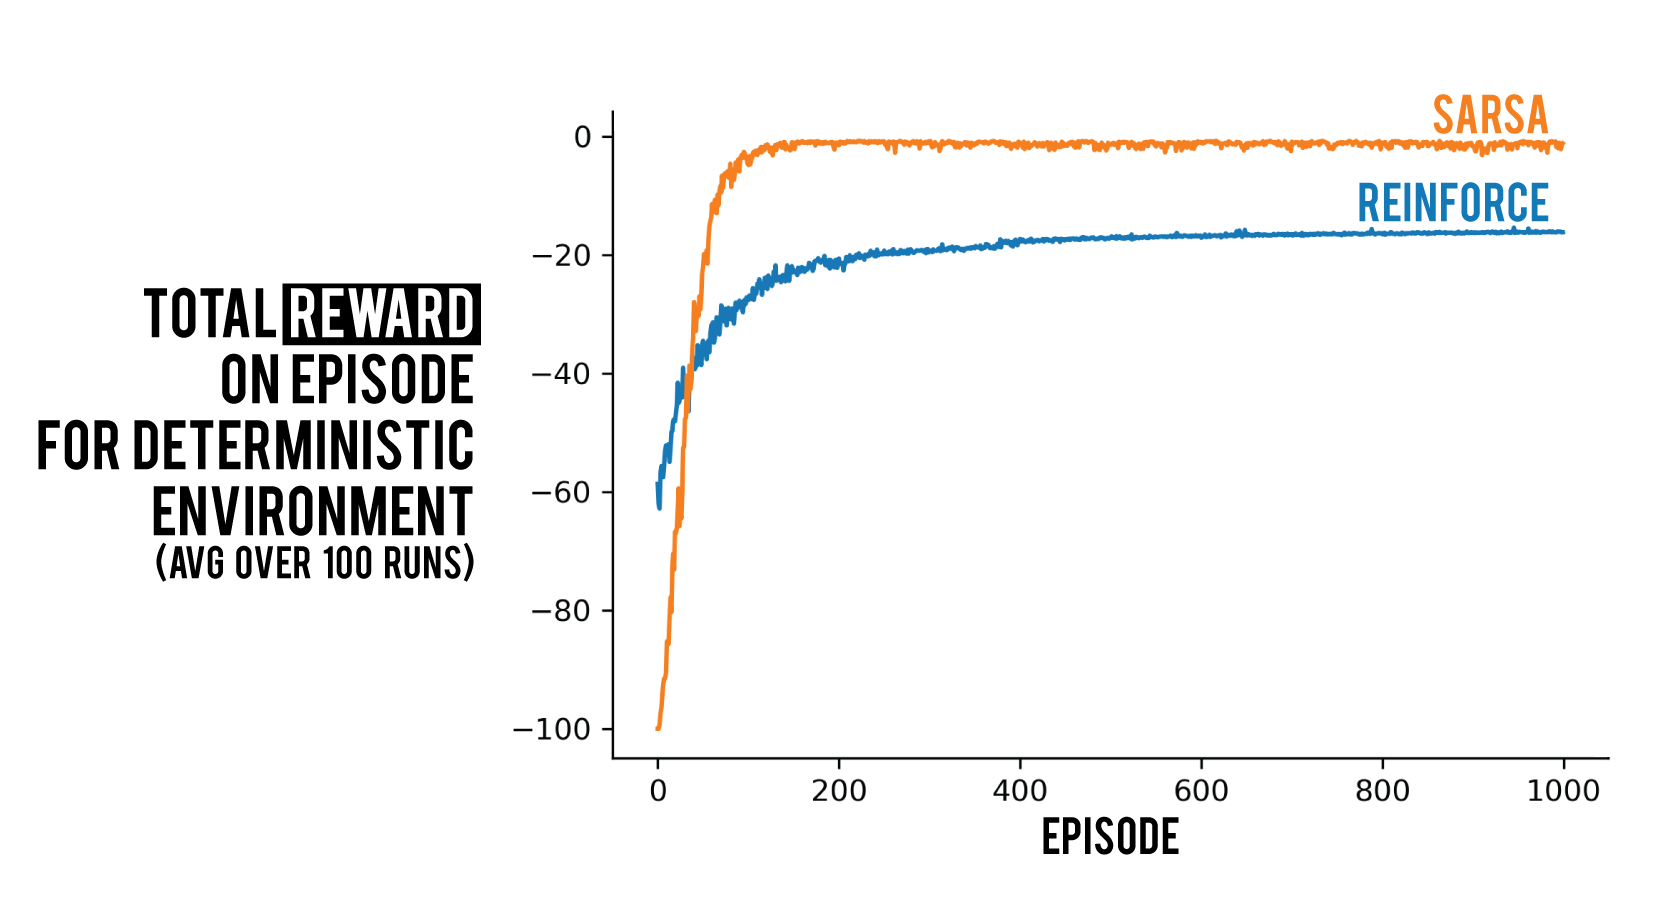
\includegraphics[width=\linewidth]{figure_deterministic}
		\caption{\small Total rewards for each episode in the deterministic environment, averaged over 100 runs. As can be seen SARSA outperformed REINFORCE with a large margin.}
		\label{fig:deterministic}
	\end{figure}
	
	Surprisingly though the next part of my hypothesis didn't prove to be true; as can be seen in the figure \ref{fig:stochastic}, SARSA still performed better than REINFORCE even though I added stochasticity to the environment. I thought this might be because I don't have enough stochasticity or too small of an environment, so I tweaked the environment a little to make sure this was not the case. 
	
	\begin{figure}[h]
		\centering
		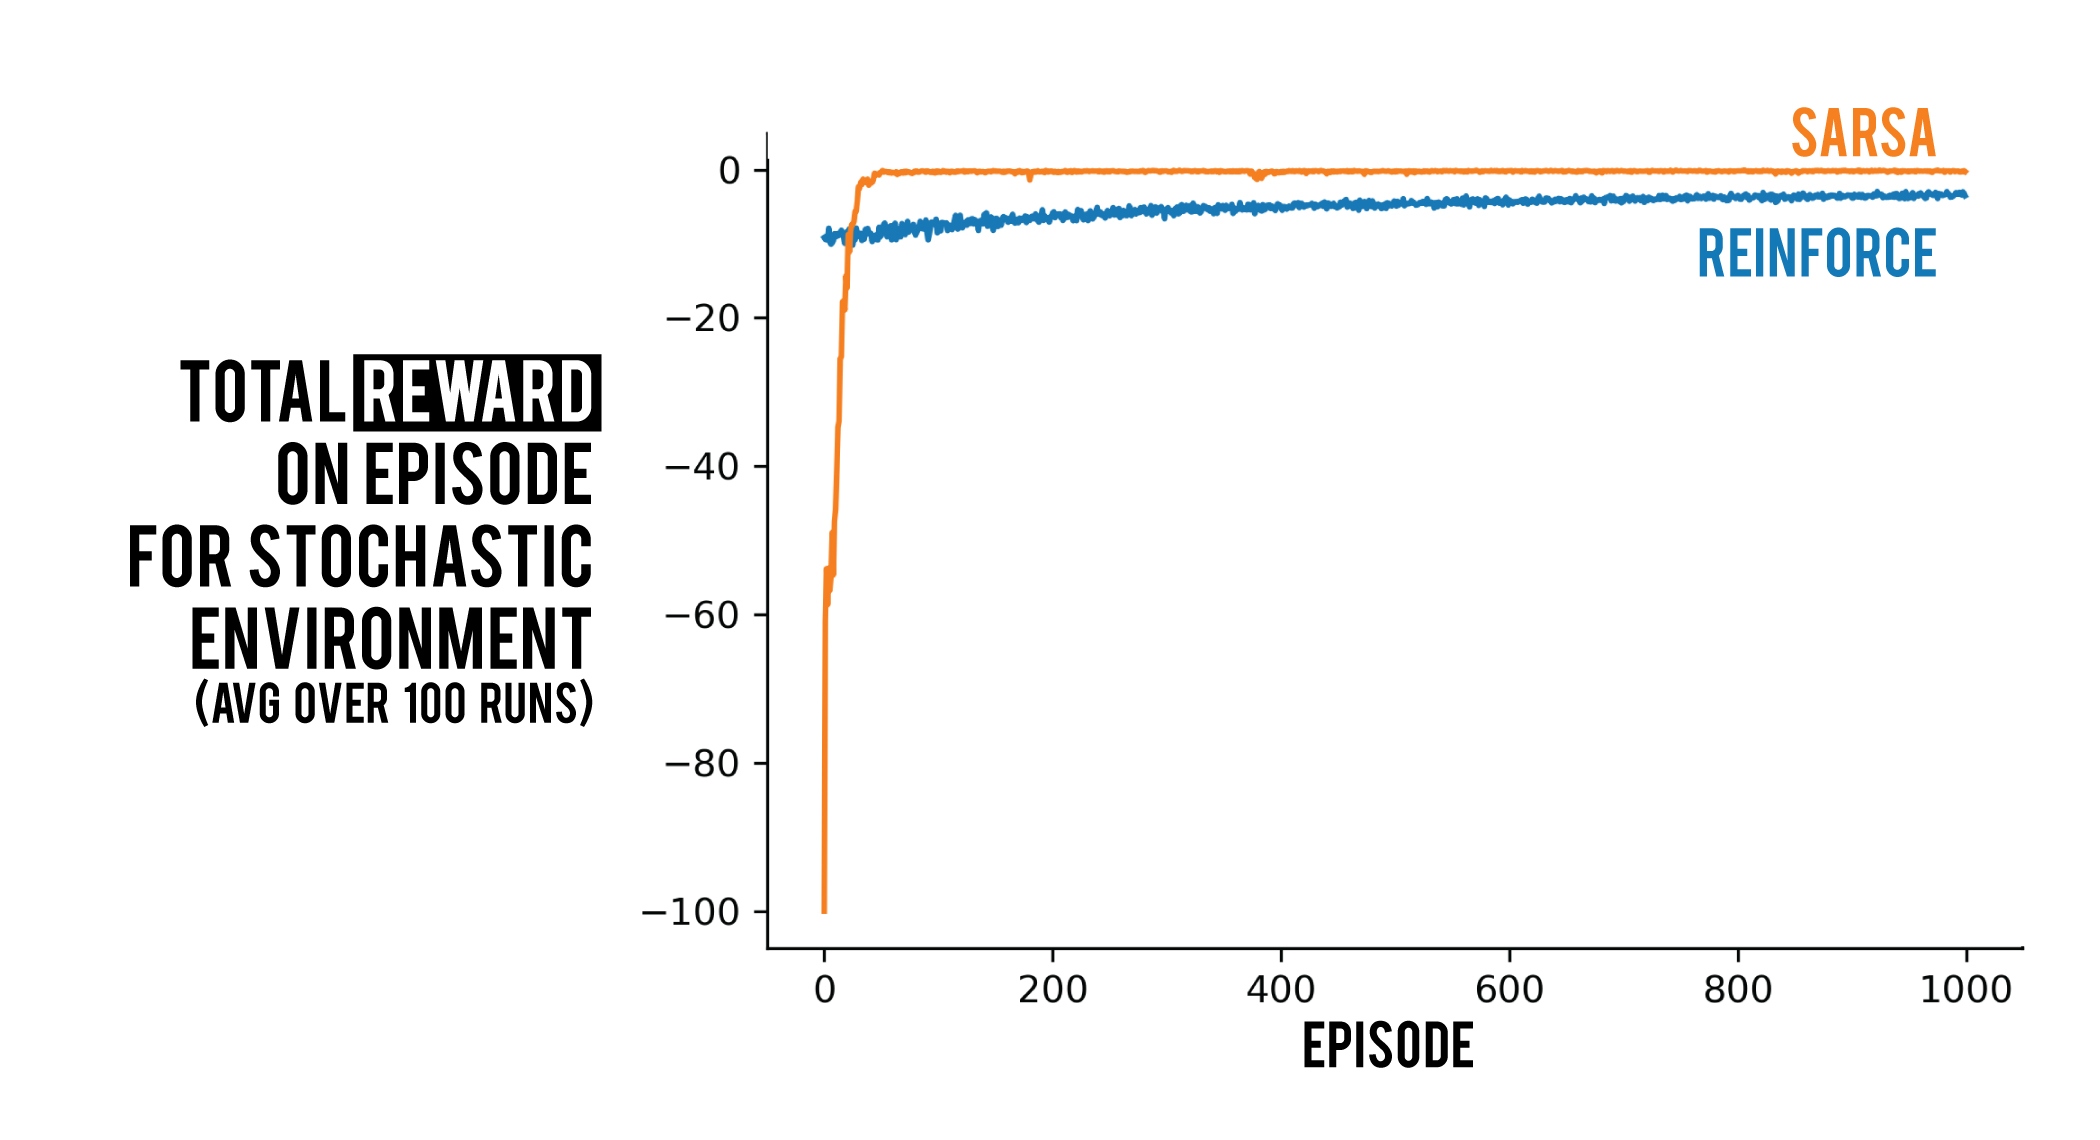
\includegraphics[width=\linewidth]{figure_stochastic}
		\caption{\small Total rewards for each episode in the stochastic environment, averaged over 100 runs. Again SARSA outperformed REINFORCE with a large margin, even though REINFORCE started off way better.}
		\label{fig:stochastic}
	\end{figure}

	\textbf{Keep trying} I added wind into the environment, that moves the agent randomly with 20\% chance (in any of the four directions) when agent tries to make a move. The results didn't change in terms of which algorithm performs better. Figure \ref{fig:wind} shows that, my concerns might have been true, so adding more stochasticity might make REINFORCE perform better compared to SARSA. I therefor created a more randomized experiment and ran it on the algorithms. \\
	
	This time I increased the random wind to 50\% chance, so the agent will move randomly half of the time. And the results in the Figure \ref{fig:wind_50} shows how two algorithms came even closer. Unfortunately due to time constraints I couldn't run more experiments to see if my expectation was definitely true. Though I currently am running a more stochastic environment and the REINFORCE is much faster for the first 50 runs that ran through, but I won't be making any claims since I don't have the actual results yet.
			
	\begin{figure}[h]
		\centering
		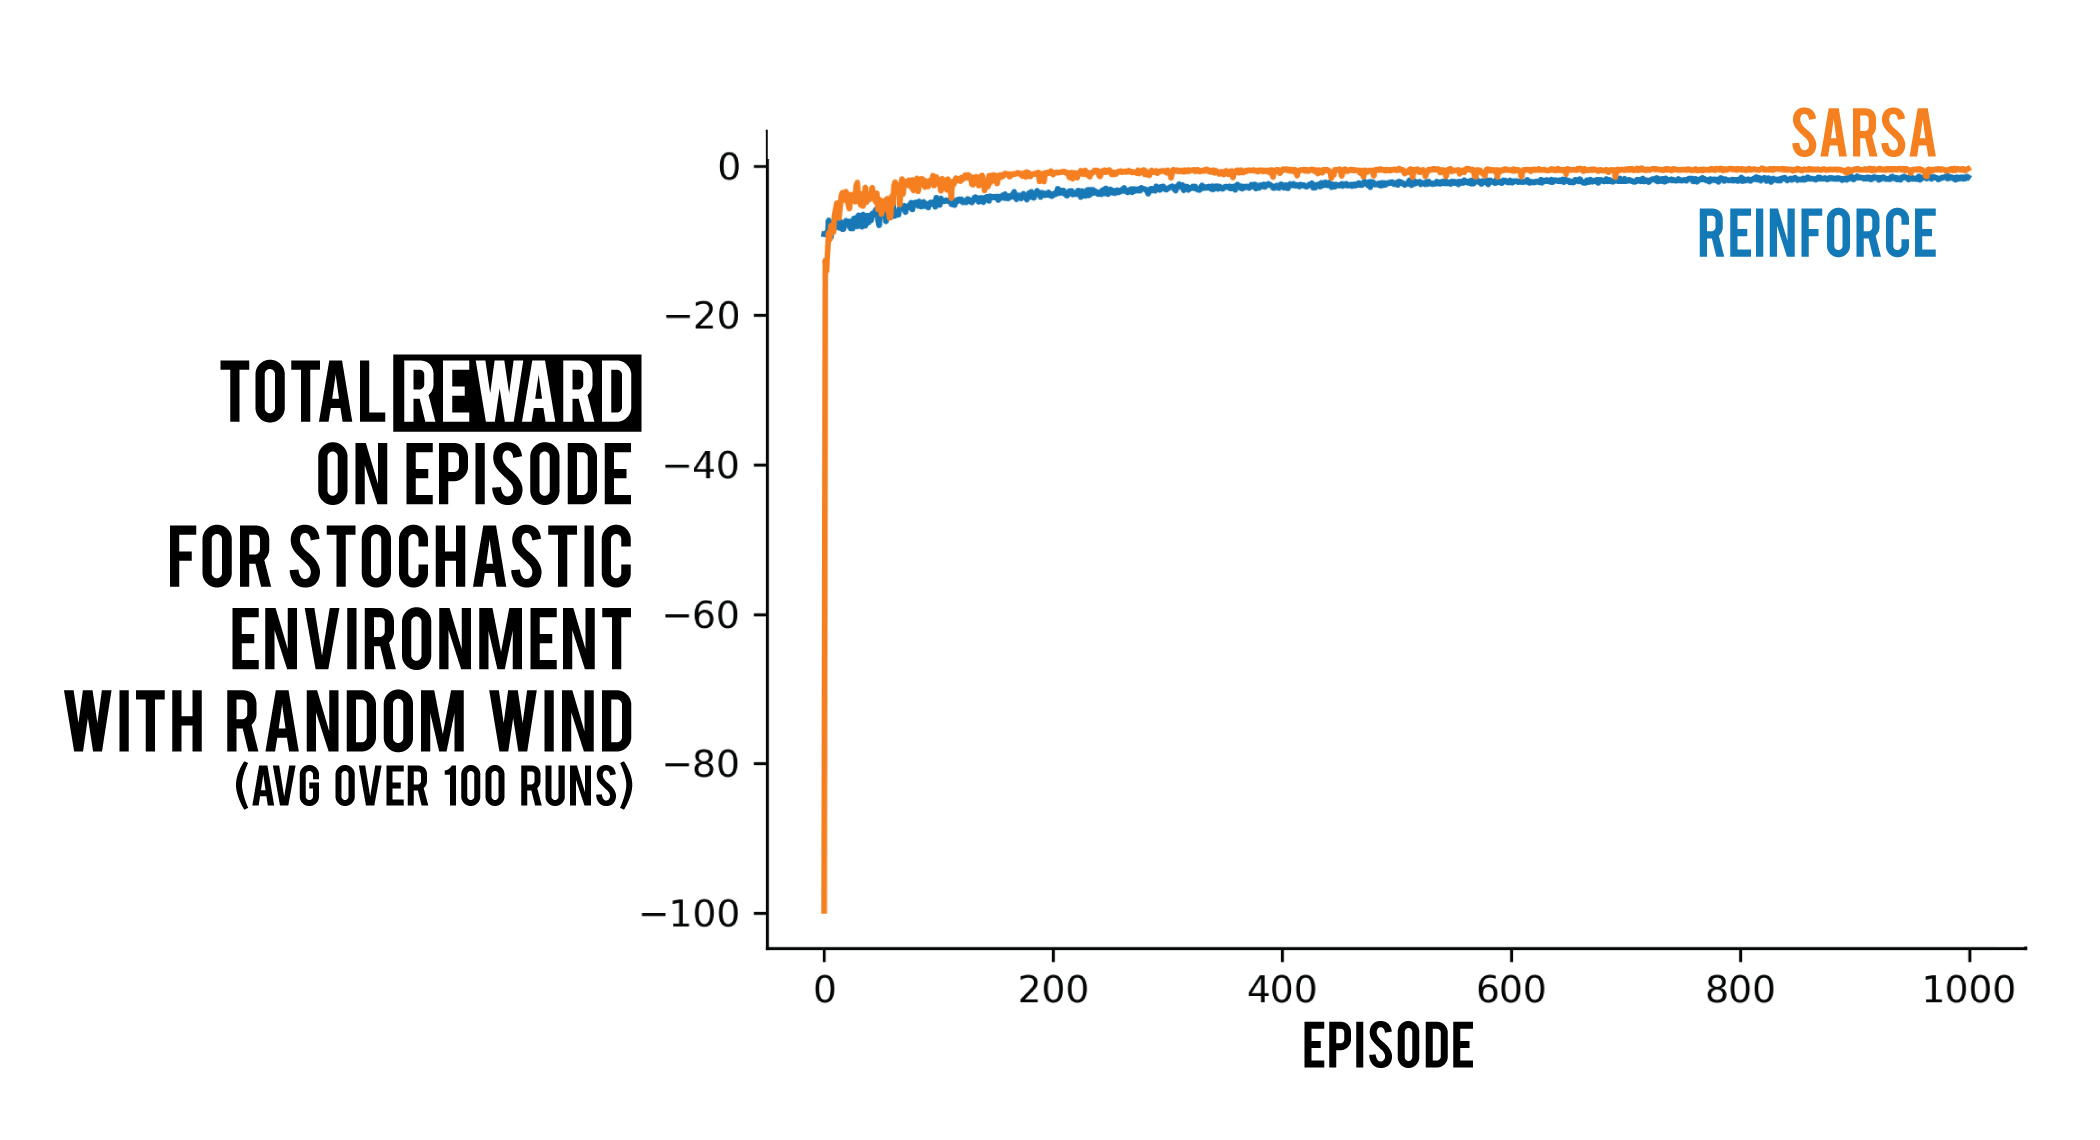
\includegraphics[width=\linewidth]{figure_wind}
		\caption{\small Total rewards for each episode in the stochastic environment with the added random wind, averaged over 100 runs. This time SARSA is better with only a small margin.}
		\label{fig:wind}
	\end{figure}

	\begin{figure}[H]
		\centering
		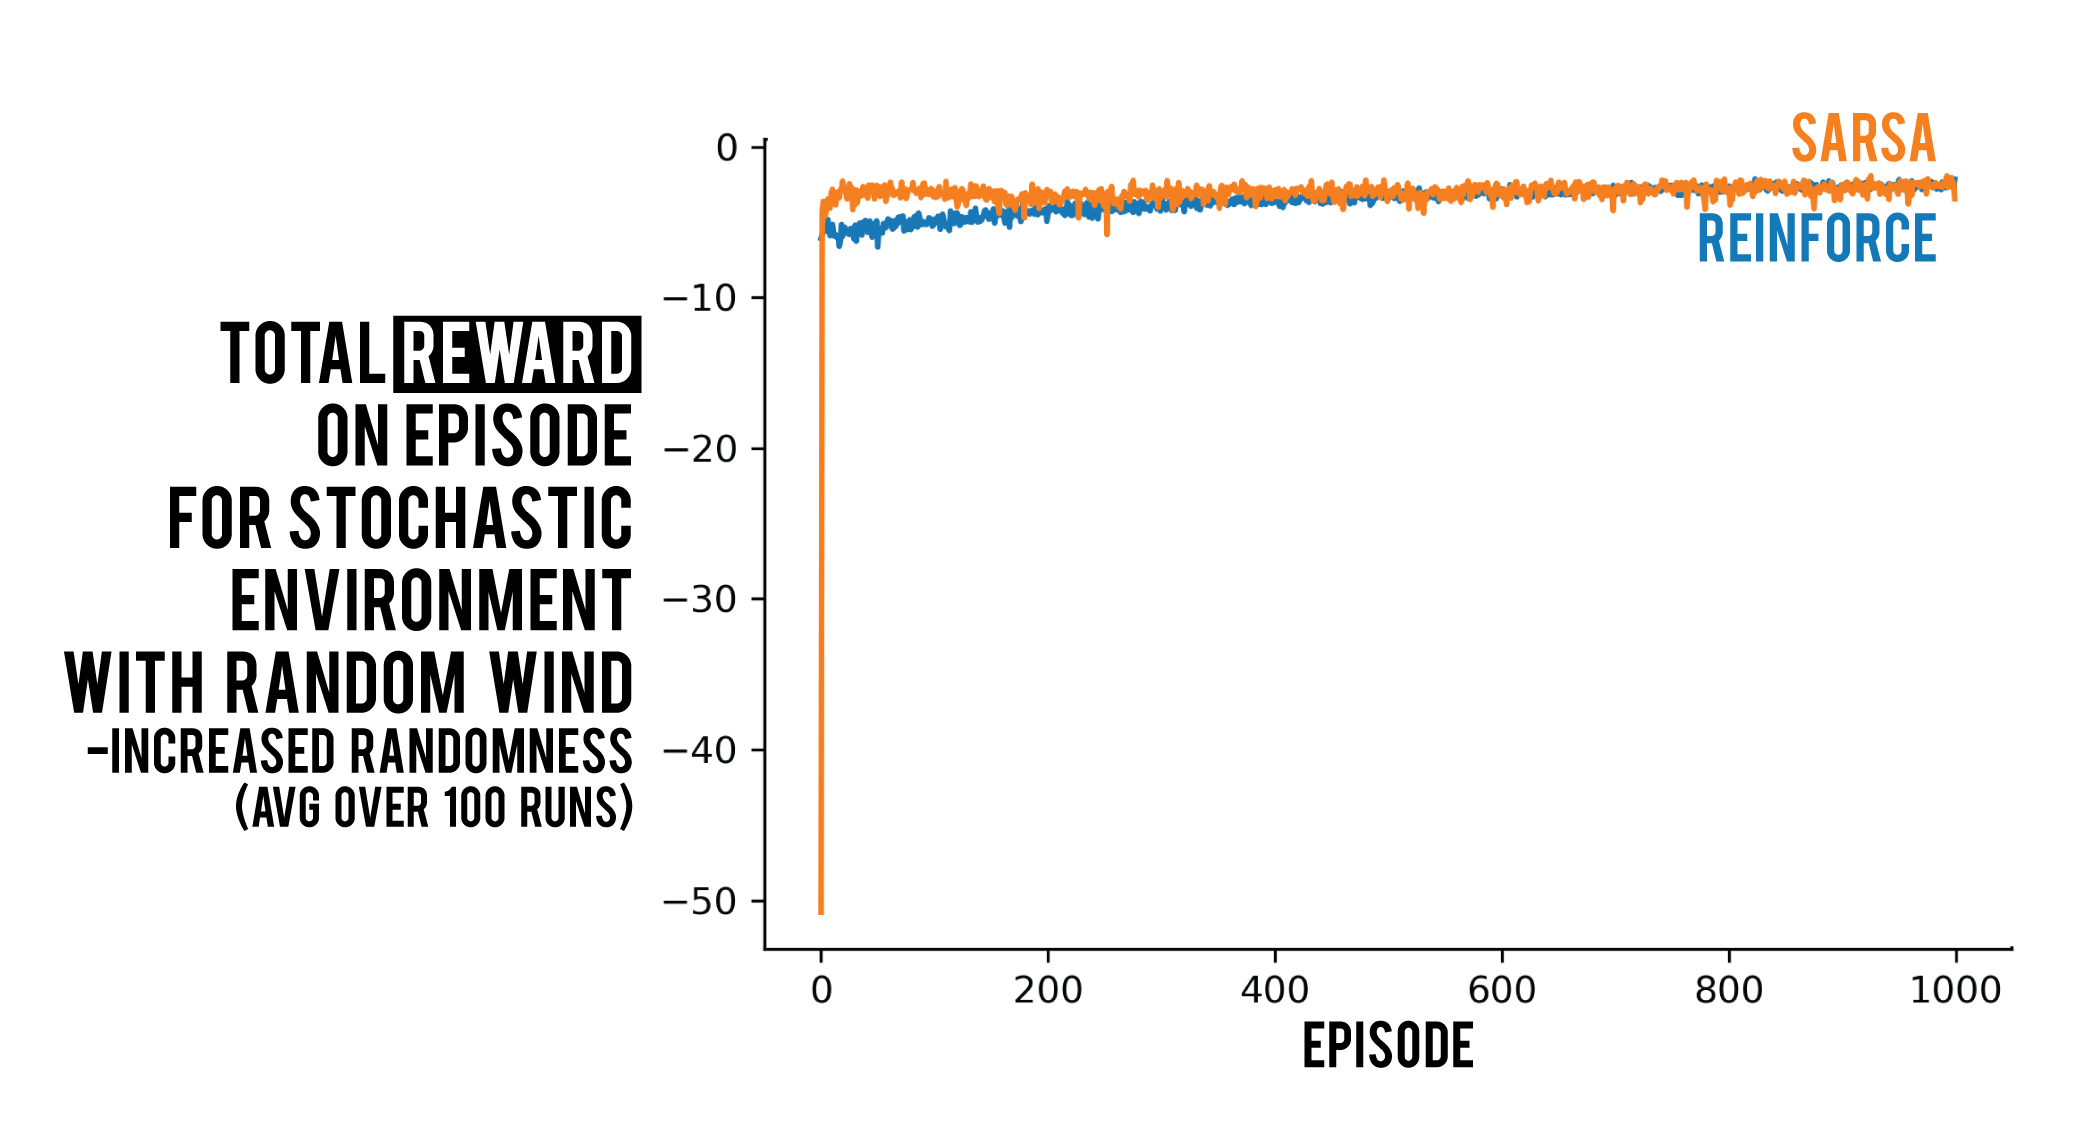
\includegraphics[width=\linewidth]{figure_wind_increased}
		\caption{\small Total rewards for each episode in the stochastic environment with the increased random wind, the chance of random action is 50\% instead of 20\% as in the plot above, averaged over 100 runs. We see that the results are the same for 1000 episodes.}
		\label{fig:wind_50}
	\end{figure}
	
	\section{Conclusion}
	
	From comparing action-value based methods and policy gradient methods in episodic cases, I finalized that as my hypothesis suggested, action-value based methods perform better in deterministic environments. As opposed to my hypothesis however, policy gradients does not seem to be performing significantly better in the stochastic environments, although as my extended studies show that this might be most probably due to limited stochasticity, and needs further investigation. \\
	
	With that being said, in every scenario SARSA outperformed REINFORCE and on top of it, even if the assumption of more stochasticity needed is true, I think my results show that SARSA, therefor action-value based methods, are very well able to find the optimal policy for the stochastic environments. So my results contradicts with the statement that value based methods are not able to find optimal policy for stochastic environments. The level of stochasticity might be of some effect, but then again, the statement should be made that there is some level of randomness that value based methods can work well.
	
	%%%%%%%%%%%%%%
	% References %
	%%%%%%%%%%%%%%
	\section{References}
	
	\noindent Williams, R. J. (1992). Simple statistical gradient-following algorithms for connectionist reinforcement learning. Machine learning, 8(3-4), 229-256\\
	
	\noindent Sutton, R. S., \& Barto, A. G. (2018). Reinforcement learning: An introduction. MIT press.
	
	
	
\end{document}